\documentclass[10pt]{article}
\usepackage[a4paper,margin=1.7cm]{geometry}
\usepackage{graphicx,booktabs,amsmath,amssymb,hyperref,xcolor,caption,enumitem,multirow}
\usepackage[T1]{fontenc}
\usepackage{lmodern}
\captionsetup{font=small,skip=2pt}
\setlist{nosep,leftmargin=*}
\setlength{\parskip}{2pt}
\setlength{\parindent}{0pt}
\graphicspath{{figures/}}
% AUTO-GENERATED by report/make_numbers.py -- do not edit by hand.
% SOURCES: data/sealed_v1_truth.json, outputs/diagnosis_null/null_tops.csv, outputs/diagnosis_sweep/data/sweep_8000_truth.json, outputs/diagnosis_sweep/data/sweep_8001_truth.json, outputs/diagnosis_sweep/data/sweep_8002_truth.json, outputs/diagnosis_sweep/data/sweep_8003_truth.json, outputs/diagnosis_sweep/data/sweep_8004_truth.json, outputs/diagnosis_sweep/data/sweep_8005_truth.json, outputs/diagnosis_sweep/data/sweep_8006_truth.json, outputs/diagnosis_sweep/data/sweep_8007_truth.json, outputs/diagnosis_sweep/data/sweep_8008_truth.json, outputs/diagnosis_sweep/data/sweep_8009_truth.json, outputs/diagnosis_sweep/data/sweep_8010_truth.json, outputs/diagnosis_sweep/data/sweep_8011_truth.json, outputs/diagnosis_sweep/data/sweep_8012_truth.json, outputs/diagnosis_sweep/data/sweep_8013_truth.json, outputs/diagnosis_sweep/data/sweep_8014_truth.json, outputs/diagnosis_sweep/data/sweep_8015_truth.json, outputs/diagnosis_sweep/data/sweep_8016_truth.json, outputs/diagnosis_sweep/data/sweep_8017_truth.json, outputs/diagnosis_sweep/data/sweep_8018_truth.json, outputs/diagnosis_sweep/data/sweep_8019_truth.json, outputs/diagnosis_sweep/data/sweep_8020_truth.json, outputs/diagnosis_sweep/data/sweep_8021_truth.json, outputs/diagnosis_sweep/sensitivity_sweep.csv, outputs/diagnosis_validation/rule_validation.csv, outputs/public/results.json, outputs/restart/restart_check.json, outputs/smoke/smoke.json, outputs/studies/ablation/ablation.json, outputs/studies/bias/bias.json, outputs/studies/coverage/coverage.json, outputs/studies/coverage/coverage_rows.csv, outputs/studies/design/design.json, outputs/studies/design/design_rows.csv, outputs/verify/verify.json, results/public_eval_v1_results.json, results/sealed_diagnosis.json
\newcommand{\OrdMin}{1.993}
\newcommand{\OrdMax}{1.999}
\newcommand{\MmsErrHundred}{3.3e-05}
\newcommand{\SteadyErr}{2.9e-06}
\newcommand{\EnergyDefect}{2e-16}
\newcommand{\ClnBad}{10}
\newcommand{\ClnConflict}{8}
\newcommand{\ClnDup}{6}
\newcommand{\ClnMissing}{5}
\newcommand{\ClnTime}{2}
\newcommand{\ClnSuspect}{6}
\newcommand{\TrueA}{0.104}
\newcommand{\TrueB}{-0.361}
\newcommand{\TrueH}{0.322}
\newcommand{\FvA}{0.107}
\newcommand{\FvALo}{0.100}
\newcommand{\FvAHi}{0.113}
\newcommand{\FvB}{-0.405}
\newcommand{\FvBLo}{-0.471}
\newcommand{\FvBHi}{-0.339}
\newcommand{\FvH}{0.330}
\newcommand{\FvHLo}{0.272}
\newcommand{\FvHHi}{0.388}
\newcommand{\FvChi}{1.12}
\newcommand{\FvStatus}{ok}
\newcommand{\FvTrainRmse}{0.0135}
\newcommand{\FvValRmse}{0.0124}
\newcommand{\FvValCov}{0.96}
\newcommand{\FvValChi}{0.93}
\newcommand{\FvFitSec}{6.1}
\newcommand{\FvTestNoisy}{0.0131}
\newcommand{\FvTestLatent}{0.0012}
\newcommand{\FvTestCovY}{0.95}
\newcommand{\FvTestCovU}{0.99}
\newcommand{\CstA}{0.120}
\newcommand{\CstALo}{0.109}
\newcommand{\CstAHi}{0.131}
\newcommand{\CstB}{0.000}
\newcommand{\CstBLo}{0.000}
\newcommand{\CstBHi}{0.000}
\newcommand{\CstH}{0.278}
\newcommand{\CstHLo}{0.215}
\newcommand{\CstHHi}{0.340}
\newcommand{\CstChi}{1.48}
\newcommand{\CstStatus}{weak\_evidence}
\newcommand{\CstTrainRmse}{0.0158}
\newcommand{\CstValRmse}{0.0142}
\newcommand{\CstValCov}{0.92}
\newcommand{\CstValChi}{1.18}
\newcommand{\CstFitSec}{5.6}
\newcommand{\CstTestNoisy}{0.0139}
\newcommand{\CstTestLatent}{0.0084}
\newcommand{\CstTestCovY}{0.95}
\newcommand{\CstTestCovU}{0.33}
\newcommand{\FvEnergy}{5e-16}
\newcommand{\LrtBeta}{150}
\newcommand{\ScanVerdict}{no fault detected}
\newcommand{\ScanTop}{3.9}
\newcommand{\PinnNSeeds}{3}
\newcommand{\PinnNFailed}{0}
\newcommand{\PinnNWeak}{3}
\newcommand{\PinnA}{0.094}
\newcommand{\PinnAMin}{0.091}
\newcommand{\PinnAMax}{0.096}
\newcommand{\PinnB}{-0.426}
\newcommand{\PinnBMin}{-0.444}
\newcommand{\PinnBMax}{-0.413}
\newcommand{\PinnH}{0.174}
\newcommand{\PinnHMin}{0.158}
\newcommand{\PinnHMax}{0.185}
\newcommand{\PinnTrainSec}{243}
\newcommand{\PinnAdaptSec}{59}
\newcommand{\PinnObsLoss}{1.16}
\newcommand{\PinnEB}{0.022}
\newcommand{\PinnCons}{0.0029}
\newcommand{\PinnDchiMin}{37}
\newcommand{\PinnDchiMax}{58}
\newcommand{\PinnDchiLim}{26.1}
\newcommand{\PinnTrainRmse}{0.0137}
\newcommand{\PinnValRmse}{0.0164}
\newcommand{\PinnTestNoisy}{0.0169}
\newcommand{\PinnTestLatent}{0.0144}
\newcommand{\PinnTestCovY}{0.04}
\newcommand{\EvalWall}{16}
\newcommand{\EvalCommit}{34320ba}
\newcommand{\EvalDirty}{False}
\newcommand{\VOneSeedTwoChi}{1.2077}
\newcommand{\VOneSeedTwoLim}{1.2078}
\newcommand{\VOneSeedTwoH}{0.185}
\newcommand{\VOneChiGap}{0.09}
\newcommand{\CovIndA}{20}
\newcommand{\CovIndB}{20}
\newcommand{\CovIndH}{20}
\newcommand{\CovIndN}{20}
\newcommand{\CovIndRawA}{20}
\newcommand{\CovIndRawB}{20}
\newcommand{\CovIndRawH}{20}
\newcommand{\CovIndWilsonLo}{0.84}
\newcommand{\CovArA}{19}
\newcommand{\CovArB}{20}
\newcommand{\CovArH}{20}
\newcommand{\CovArN}{20}
\newcommand{\CovArRawA}{18}
\newcommand{\CovArRawB}{18}
\newcommand{\CovArRawH}{15}
\newcommand{\CovArWilsonLo}{0.76}
\newcommand{\CovIndFlagged}{0}
\newcommand{\CovArFlagged}{20}
\newcommand{\RedrawRatioH}{1.29}
\newcommand{\RedrawRatioA}{1.25}
\newcommand{\AbBaseA}{0.070}
\newcommand{\AbBaseAW}{0.007}
\newcommand{\AbBaseB}{0.398}
\newcommand{\AbBaseBW}{0.168}
\newcommand{\AbBaseH}{0.239}
\newcommand{\AbBaseHW}{0.045}
\newcommand{\AbBaseLat}{0.0012}
\newcommand{\AbBaseStatus}{ok}
\newcommand{\AbEarlyA}{0.065}
\newcommand{\AbEarlyAW}{0.025}
\newcommand{\AbEarlyB}{0.217}
\newcommand{\AbEarlyBW}{0.496}
\newcommand{\AbEarlyH}{0.193}
\newcommand{\AbEarlyHW}{0.236}
\newcommand{\AbEarlyLat}{0.0060}
\newcommand{\AbEarlyStatus}{weak\_evidence}
\newcommand{\AbSparseA}{0.073}
\newcommand{\AbSparseAW}{0.014}
\newcommand{\AbSparseB}{0.491}
\newcommand{\AbSparseBW}{0.306}
\newcommand{\AbSparseH}{0.228}
\newcommand{\AbSparseHW}{0.072}
\newcommand{\AbSparseLat}{0.0015}
\newcommand{\AbSparseStatus}{ok}
\newcommand{\AbNoRightA}{0.069}
\newcommand{\AbNoRightAW}{0.009}
\newcommand{\AbNoRightB}{0.379}
\newcommand{\AbNoRightBW}{0.207}
\newcommand{\AbNoRightH}{0.304}
\newcommand{\AbNoRightHW}{0.237}
\newcommand{\AbNoRightLat}{0.0018}
\newcommand{\AbNoRightStatus}{weak\_evidence}
\newcommand{\AbNoLeftA}{0.070}
\newcommand{\AbNoLeftAW}{0.008}
\newcommand{\AbNoLeftB}{0.387}
\newcommand{\AbNoLeftBW}{0.250}
\newcommand{\AbNoLeftH}{0.240}
\newcommand{\AbNoLeftHW}{0.047}
\newcommand{\AbNoLeftLat}{0.0015}
\newcommand{\AbNoLeftStatus}{ok}
\newcommand{\AbConstAA}{0.062}
\newcommand{\AbConstAAW}{0.007}
\newcommand{\AbConstAB}{0.000}
\newcommand{\AbConstABW}{0.000}
\newcommand{\AbConstAH}{0.249}
\newcommand{\AbConstAHW}{0.057}
\newcommand{\AbConstALat}{0.0111}
\newcommand{\AbConstAStatus}{ok}
\newcommand{\AbZeroOffA}{0.074}
\newcommand{\AbZeroOffAW}{0.019}
\newcommand{\AbZeroOffB}{0.700}
\newcommand{\AbZeroOffBW}{0.388}
\newcommand{\AbZeroOffH}{0.184}
\newcommand{\AbZeroOffHW}{0.073}
\newcommand{\AbZeroOffLat}{0.0060}
\newcommand{\AbZeroOffStatus}{weak\_evidence}
\newcommand{\AbTrueA}{0.07}
\newcommand{\AbTrueB}{0.45}
\newcommand{\AbTrueH}{0.25}
\newcommand{\AbHWidthRatioRight}{5.3}
\newcommand{\AbHWidthRatioEarly}{5.3}
\newcommand{\AbLatRatioConst}{9}
\newcommand{\BiasOkTrain}{0.0105}
\newcommand{\BiasOkLat}{0.0012}
\newcommand{\BiasOkBErr}{0.013}
\newcommand{\BiasOkChi}{0.98}
\newcommand{\BiasWrongTrain}{0.0150}
\newcommand{\BiasWrongLat}{0.0175}
\newcommand{\BiasWrongBErr}{0.600}
\newcommand{\BiasWrongChi}{2.09}
\newcommand{\BiasZeroOffTrain}{0.0228}
\newcommand{\BiasZeroOffLat}{0.0052}
\newcommand{\BiasZeroOffBErr}{0.083}
\newcommand{\BiasZeroOffChi}{5.03}
\newcommand{\DesBaseHW}{0.0531}
\newcommand{\DesAHW}{0.0376}
\newcommand{\DesBHW}{0.0487}
\newcommand{\DesAWins}{10}
\newcommand{\DesN}{10}
\newcommand{\DesRuleA}{10}
\newcommand{\DesAErr}{0.0078}
\newcommand{\DesBErr}{0.0072}
\newcommand{\DiagValOk}{12}
\newcommand{\DiagValN}{12}
\newcommand{\SweepNamed}{13}
\newcommand{\SweepNamedWrong}{0}
\newcommand{\SweepN}{22}
\newcommand{\SweepDetected}{13}
\newcommand{\SweepAmbig}{1}
\newcommand{\SweepVOneMiss}{2}
\newcommand{\SweepMissBetaErr}{0.09}
\newcommand{\SweepMissDrift}{0.01}
\newcommand{\SweepMissQ}{0.03}
\newcommand{\SweepMissBias}{0.02}
\newcommand{\NullMax}{6.8}
\newcommand{\NullN}{13}
\newcommand{\NullFalse}{0}
\newcommand{\SealVerdict}{suspected:heat source}
\newcommand{\SealDchi}{38}
\newcommand{\SealQ}{0.051}
\newcommand{\SealQsd}{0.009}
\newcommand{\SealBaseH}{0.178}
\newcommand{\SealTrueQ}{0.082}
\newcommand{\SealTrueXc}{0.78}
\newcommand{\SealTrueH}{0.288}
\newcommand{\SealHeatRatio}{6}
\newcommand{\SealFixedH}{0.279}
\newcommand{\RestartDiff}{0}
\newcommand{\RestartAll}{all pass}
\newcommand{\SmokeSec}{205}
\newcommand{\SmokeMin}{3.4}
\newcommand{\SmokeOk}{PASS}

\newcommand{\syn}{\textsuperscript{\textsc{syn}}}

\title{\vspace{-1.2cm}Inverse Heat Modelling and Scientific Diagnostics\\\large AI/ML Engineer Intern take-home --- report}
\author{Adit Unnikrishnan}
\date{25 October 2026 \quad (code: \texttt{github.com/aua27/ShodhAI\_Assignment}, commit \texttt{\EvalCommit})}

\begin{document}
\maketitle
\vspace{-0.8cm}

\paragraph{Data status (read first).} Only the assignment PDF was received; the versioned data
bundle and the Stage-4 diagnosis dataset were not attached (requested by email). Every result below
is therefore on \textbf{synthetic} data generated to the schema the brief describes, with ground
truth stored separately and read only for scoring; such numbers carry the mark~\syn. The pipeline
takes any bundle in the documented format (README), so a real bundle needs a one-line config change.

\section{Formulation}
\textbf{Model.} $u_t=\partial_x[a(x)u_x]$, $a=a_0e^{\beta(2x-1)}$, $u(0,t)=g(t)$,
$-a(1)u_x(1,t)=h[u(1,t)-T_a(t)]$, readings $y=u(x_s,t)+b_s+\varepsilon$, $b_{\rm ref}=0$. Physically:
Fourier conduction with a graded conductivity ($a_0$ = mid-rod value, $e^{2\beta}$ = right/left
ratio), a clamped heater at $x{=}0$ and Newton cooling at $x{=}1$. With $a\approx0.07$ heat travels
$\sqrt{at}\approx0.26$ in the experiment, so the Robin end is seen mainly by the right-most sensors:
the a-priori reason $h$ is the hardest parameter. Heat leaving at $x{=}1$ crosses conduction and film
resistances in series, so $a_0$, $h$ and offsets can trade off.

\textbf{Inverse problem.} $\theta=(a_0,\beta,h,b_s)$, all box-constrained to the brief's ranges;
minimise $\tfrac12\sum_k[(u_k(\theta)+b_{s(k)}-y_k)/\sigma_k]^2$ (Gaussian likelihood with the
supplied noise sd). Offsets are \emph{persistent} per sensor across experiments, enter linearly
(exact Jacobian columns), and the reference sensor anchors the level (without it offsets and smooth
physics changes exchange misfit). Uncertainty: Gauss--Newton/Laplace covariance $(J^\top J)^{-1}$ ---
local, linearised, conditional on the model --- with guards (\S5) that widen or withhold it.
\textbf{Assumptions:} independent Gaussian noise with known sd (tested: residual autocorrelation),
model form correct (tested: nested-model and fault tests), piecewise-linear inputs.
\textbf{Data audit.} Rows are cleaned explicitly and logged with their raw CSV line: in the public
bundle\syn\ \ClnBad\ \texttt{bad}-flagged, \ClnConflict\ conflicting repeated-ID, \ClnDup\ exact
duplicate, \ClnMissing\ missing and \ClnTime\ out-of-domain rows were dropped; \ClnSuspect\
\texttt{suspect} rows kept and logged. Identity key $=$(experiment, obs\_id); conflicting copies are
all dropped (no silent tie-break). Split: fit E1--E3, validate E4 (labels never reach a fitting
routine --- tested by corrupting them), predict E5 from inputs only.

\section{Stage 1 --- reference solver and inference}
Cell-centred finite volumes with exact face diffusivities (conservative: energy changes only through
boundary fluxes), the Robin end as half-cell conduction in series with $h$, Crank--Nicolson with
Rannacher start-up (four backward-Euler quarter steps; avoids CN ringing when $f(0)\neq g(0)$).
\textbf{Independent verification:} (i) manufactured solution with a hand-derived source --- observed
order \OrdMin--\OrdMax\ under joint space--time refinement (Fig.~\ref{fig:ver}a), RMSE \MmsErrHundred\ at
the production grid (100 cells, 400 steps) vs noise $\approx10^{-2}$; (ii) steady state against the closed
form, error \SteadyErr; (iii) discrete energy balance to \EnergyDefect; (iv) maximum principle with a
discontinuous corner. Synthetic data are generated on a $4\times$ finer grid than inference (no
``inverse crime''). Fitting: bounded trust-region least squares, multistart (Latin hypercube), central
differences for $(a_0,\beta,h)$. Known-parameter recovery is a test on separate synthetic data (all
three within $4\sigma$, offsets within 0.01); coverage over 20 datasets is in \S4.

\begin{table}[t]\small\centering
\caption{Public bundle\syn: estimates (95\% Laplace intervals) and errors. Truth $a_0{=}\TrueA$,
$\beta{=}\TrueB$, $h{=}\TrueH$. ``noisy'' = vs readings $y$; ``latent'' = vs noise-free $u$ at E5
queries. PINN: mean over \PinnNSeeds\ seeds, [min,max] across seeds (a spread, \emph{not} an interval).}
\label{tab:main}
\begin{tabular}{lccc}\toprule
 & FV, variable $a(x)$ (primary) & FV, constant $a$ (baseline) & inverse PINN\\\midrule
$a_0$ & \FvA\ [\FvALo, \FvAHi] & \CstA\ [\CstALo, \CstAHi] & \PinnA\ [\PinnAMin, \PinnAMax]\\
$\beta$ & \FvB\ [\FvBLo, \FvBHi] & 0 (fixed) & \PinnB\ [\PinnBMin, \PinnBMax]\\
$h$ & \FvH\ [\FvHLo, \FvHHi] & \CstH\ [\CstHLo, \CstHHi] & \PinnH\ [\PinnHMin, \PinnHMax]\\
$\chi^2_\nu$ (train) & \FvChi & \CstChi & --- \\
train RMSE (noisy) & \FvTrainRmse & \CstTrainRmse & \PinnTrainRmse\\
val E4 RMSE (noisy) / 95\% cover. & \FvValRmse\ / \FvValCov & \CstValRmse\ / \CstValCov & \PinnValRmse\ / ---\\
test E5 RMSE noisy / latent\syn & \FvTestNoisy\ / \FvTestLatent & \CstTestNoisy\ / \CstTestLatent & \PinnTestNoisy\ / \PinnTestLatent\\
test latent-interval coverage\syn & \FvTestCovU & \CstTestCovU & ---\\
fit time (laptop CPU) & \FvFitSec\,s & \CstFitSec\,s & \PinnTrainSec\,s/seed + \PinnAdaptSec\,s adapt.\\
energy-balance defect & \FvEnergy\ (discrete) & --- & \PinnEB\ (relative)\\
status (automatic) & \FvStatus & \CstStatus & \PinnNWeak/\PinnNSeeds\ weak\_evidence\\\bottomrule
\end{tabular}
\end{table}

\textbf{Result (Table~\ref{tab:main}).} The variable model recovers all three parameters inside their
intervals with $\chi^2_\nu{=}\FvChi$. The constant baseline is the cautionary case: its error against
noisy readings is close to the primary (\CstTestNoisy\ vs \FvTestNoisy) yet its latent error is
\CstTestLatent\ vs \FvTestLatent\ and its latent intervals cover the truth only \CstTestCovU\ of the
time --- offsets absorb the missing gradient. It is rejected automatically by the nested test
($\Delta\chi^2{=}\LrtBeta$, \S5).

\section{Stage 2 --- inverse PINN}
\textbf{Design.} One $4{\times}48$ tanh MLP per experiment (inputs scaled to $[-1,1]$); shared
$(a_0,\beta,h)$ bounded by sigmoids, offsets by $0.03\tanh$. Losses in noise units (divided by the
median sensor variance) so a constraint violated by one noise level costs about one misfitted reading:
$L_{\rm obs}$ (whitened), $L_{\rm pde}$ with the \emph{conservative} operator by autograd
(flux $=a(x)u_x$, then $\partial_x$flux --- the $a'(x)u_x$ term appears automatically; unit-tested against the
hand-derived MMS source to $10^{-10}$), $L_{\rm ic}$, $L_{\rm bc}$ (Dirichlet + Robin). Uniform
collocation (2000/experiment) resampled every 250 Adam steps, then L-BFGS on a \emph{fixed} set
(resampling breaks its line search). Adam lr decays $10\times$; physics frozen for 1500 warm-up steps.
Unseen experiments: physics-only adaptation (fresh field net, PDE+IC+BC, parameters frozen; timed: \PinnAdaptSec\,s/seed).

\textbf{Development (dev bundle, one change per trial; \texttt{docs/evidence}).} (1) no warm-up: $h$
collapsed onto its bound --- an untrained field makes the Robin term cheapest at $h\to0$ and the
sigmoid saturates; (2) warm-up: $a_0,\beta$ correct, $h$ $3\times$ low with the right-most offset
absorbing it; (3) $w_{\rm bc}{=}10$: hypothesis ``BC weight pins $h$'' \textbf{refuted} ($h$ worse);
(4) $2\times$ steps: marginal; (5) $w_{\rm pde}{=}10$: worse (stiffer). Mechanism: soft constraints
tolerate $\sim$1 noise level of physics error, enough for the field to bend between the last sensor
($x{=}0.85$) and the Robin end so a wrong $h$ satisfies the BC. Tuning stopped there.

\textbf{Result.} On the public bundle\syn\ the PINN reproduces the readings ($L_{\rm obs}{=}\PinnObsLoss$,
train RMSE \PinnTrainRmse) and has small seed spread, but $h{=}\PinnH$ vs \TrueH; seed spread is
\emph{not} uncertainty. Agreement of the PINN field with an FV field at the PINN's own parameters
(RMSE \PinnCons) shows consistency only. The accuracy question is answered by an exact-physics
likelihood-ratio check (\S5): all seeds lie outside the FV fit's joint 99.9\% region
($\Delta\chi^2$ \PinnDchiMin--\PinnDchiMax\ vs \PinnDchiLim) and are reported \texttt{weak\_evidence}.
\textbf{Conclusion:} the PINN does not outperform the numerical baseline here; the FV fit is primary.

\begin{figure}[t]\centering
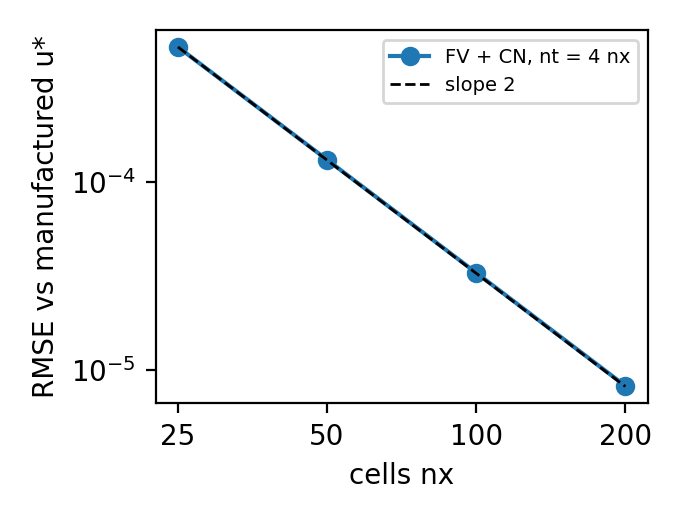
\includegraphics[width=0.27\linewidth]{refinement}\hfill
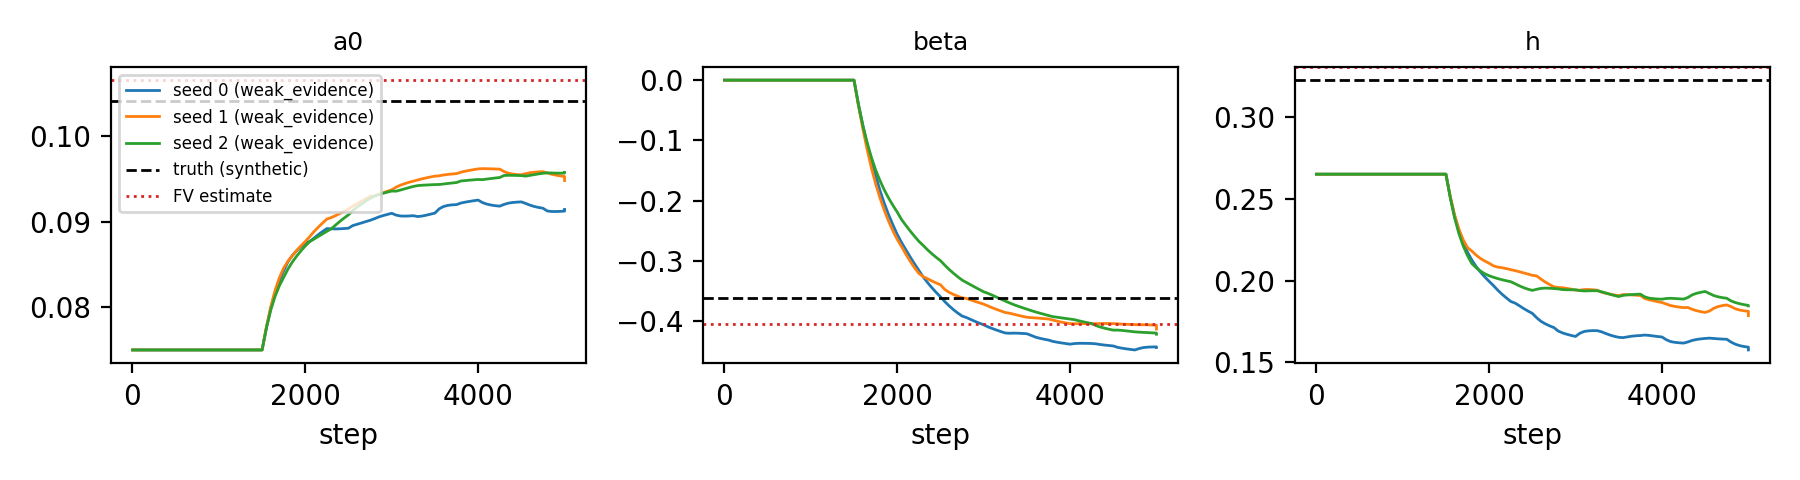
\includegraphics[width=0.70\linewidth]{pinn_traces}
\caption{(a) MMS refinement, slope 2. (b) PINN parameter trajectories, public bundle\syn, 3 seeds:
$a_0,\beta$ settle near truth (dashed) and FV (dotted); $h$ does not.}\label{fig:ver}
\end{figure}

\section{Stage 3 --- investigation}
\textbf{Uncertainty (Fig.~\ref{fig:s3}b).} 95\% Laplace intervals for $a_0,\beta,h$ on \CovIndN\
independent synthetic datasets: coverage \CovIndA/\CovIndN, \CovIndB/\CovIndN, \CovIndH/\CovIndN\
(Wilson lower bound \CovIndWilsonLo; $n$ is small --- a sanity check, not calibration). Data
uncertainty isolated by redrawing only the noise 20 times: empirical sd / Laplace sd $=$
\RedrawRatioA\ ($a_0$), \RedrawRatioH\ ($h$), within the $\pm16\%$ sampling error of an sd from 20
draws. Seed variability is a separate quantity: zero for the deterministic FV fit (multistarts agree),
the PINN spread in Table~\ref{tab:main} for the PINN. Dependence assumption tested with AR(1) noise
($\rho{=}0.6$): before the autocorrelation guard coverage fell to 90/90/75\%; with it every such
dataset is flagged (\CovArFlagged/\CovArN) and intervals widened by $(1{+}\hat\rho)/(1{-}\hat\rho)$,
restoring \CovArA/\CovArN, \CovArB/\CovArN, \CovArH/\CovArN; \CovIndFlagged/\CovIndN\ independent-noise datasets flagged.

\textbf{Controlled experiments (Fig.~\ref{fig:s3}a; one change each, fixed evaluation = latent RMSE on held-out E4).}
Truth $(\AbTrueA,\AbTrueB,\AbTrueH)$. \emph{Coverage:} removing sensors at $x\ge0.7$ widens the $h$
interval $\AbHWidthRatioRight\times$; early times only ($t\le0.3$) widen it $\AbHWidthRatioEarly\times$ and
$\beta$'s too; 4$\times$ sparser sampling widens all but stays unbiased; dropping left sensors barely
matters. \emph{Assumptions:} constant $a$ gives $\AbLatRatioConst\times$ the held-out latent error;
offsets forced to zero push $\beta$ to \AbZeroOffB. Hypotheses were stated before running (code, \texttt{ABLATION\_HYPOTHESES}).

\textbf{Experimental design.} One new sensor at $x{=}0.95$ (24 readings/experiment, unknown offset) vs
the same 24 readings spread over existing sensors. Rule, fixed before truth: choose the design with
the smaller linearised posterior sd of $h$ at a \emph{pilot} fit (Fisher information incl.\ the new
offset). The ambiguity addressed is the $h$--conduction--offset trade-off at the Robin end. The rule
chose the new sensor in \DesRuleA/\DesN\ datasets; it narrowed the $h$ interval in \DesAWins/\DesN\
(mean width \DesAHW\ vs \DesBHW; base \DesBaseHW) but mean $|h|$ error did not measurably differ at
$n{=}\DesN$ (\DesAErr\ vs \DesBErr) --- a precision gain, not a demonstrated accuracy gain.

\begin{figure}[t]\centering
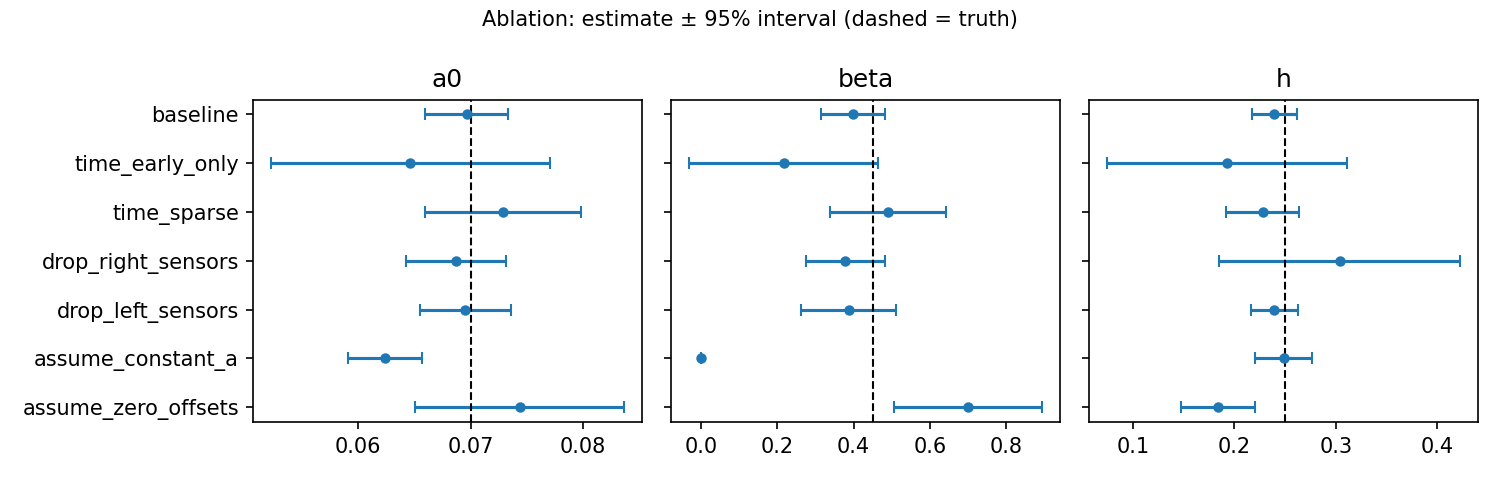
\includegraphics[width=0.62\linewidth]{ablation}\hfill
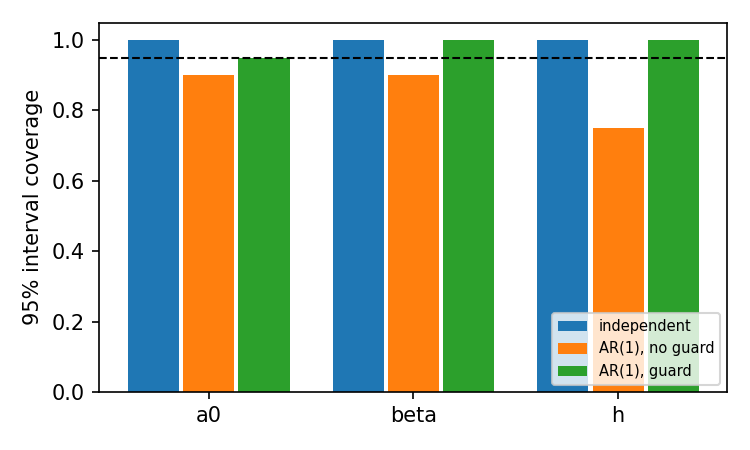
\includegraphics[width=0.36\linewidth]{coverage}
\caption{(a) Ablation: estimates $\pm$95\% (dashed: truth). (b) Interval coverage, independent vs AR(1) noise (with guard).}\label{fig:s3}
\end{figure}

\textbf{The three questions.}
\emph{Can sensor bias mask incorrect physics despite low temperature error?} Yes. On 5 strongly
graded datasets\syn\ the constant-$a$ model with free offsets reaches train RMSE \BiasWrongTrain\ (correct
model \BiasOkTrain) while $\beta$ is off by \BiasWrongBErr\ and held-out latent error is
\BiasWrongLat\ vs \BiasOkLat; on milder gradients (ablation) its $\chi^2_\nu$ looks acceptable.
Detection needs model comparison or held-out prediction, not training fit.
\emph{Which parameters become weakly identifiable?} $h$ first (right-end coverage or late times),
then $\beta$ (early times); $a_0$ stays well determined.
\emph{Which additional measurement helps, and why?} A sensor near the Robin end: it observes the
boundary gradient directly, breaking the $h$/conduction/offset trade-off --- but it brings its own
unknown offset, which the selection rule accounts for.

\section{Stage 4 --- reliability, diagnosis, recovery}
\textbf{Automatic status.} Every result carries \texttt{ok}/\texttt{weak\_evidence}/\texttt{failed}
from rules fixed in code, none using truth: $\chi^2_\nu$ above $1{+}3\sqrt{2/\nu}$; positive residual
autocorrelation ($z{>}3$); held-out predictive $\chi^2$; nested LRT constant-vs-variable $a$
($p{=}10^{-3}$); interval $>$50\% of the admissible range $\Rightarrow$ estimate \emph{withheld};
estimate on a bound; multistart disagreement; PINN exact-physics recheck; fault-hypothesis scan.
Each was added in response to a measured miss, and its false-alarm rate measured on correct models.

\textbf{Model diagnosis.} Rules frozen in \texttt{configs/diagnosis\_rules.yaml}. Observations
(residual trends, $\chi^2$, early/late parameter shift) are reported separately from causal
hypotheses, each a nested one-parameter model: drift of sensor $s$ ($y{+}rt$, every sensor),
Gaussian heat source (centre scanned), constant bias of the recorded $g$. Evidence $=\Delta\chi^2$
(LRT), with the extra parameter's estimate $\pm$ sd as sensitivity. Threshold v2 $=15.1$ (Bonferroni
over 10 hypotheses, family $p{=}10^{-3}$; v1's ad-hoc 25 missed drifts at $\Delta\chi^2$ 16--24); max over
\NullN\ fault-free bundles \NullMax. Validation\syn: \DiagValOk/\DiagValN\ correct; fault-size sweep: \SweepDetected/\SweepN\ detected,
\SweepNamedWrong\ of \SweepNamed\ named verdicts wrong. Below the limits (drift $\lesssim$0.02/unit time,
boundary bias $\lesssim$0.02) faults go undetected yet can bias $\beta$ by up to $\sim$0.09.
\textbf{Blind test:} rules committed $\rightarrow$ sealed bundle (fault drawn from OS randomness, truth
hashed) committed $\rightarrow$ verdict committed $\rightarrow$ unsealed. Verdict: \emph{\SealVerdict}
($\Delta\chi^2{=}\SealDchi$, $Q{=}\SealQ\pm\SealQsd$ at the nearest scanned centre); truth: heat source,
$Q{=}\SealTrueQ$ at $x{=}\SealTrueXc$ (width differs; integrated heat agrees within 10\%). The base fit
there reported \texttt{ok} with $h{=}\SealBaseH$ (true \SealTrueH; \SealFixedH\ once the source is
modelled) --- which is why the fault scan now runs inside \texttt{evaluate} (public bundle: \ScanVerdict).

\begin{figure}[t]\centering
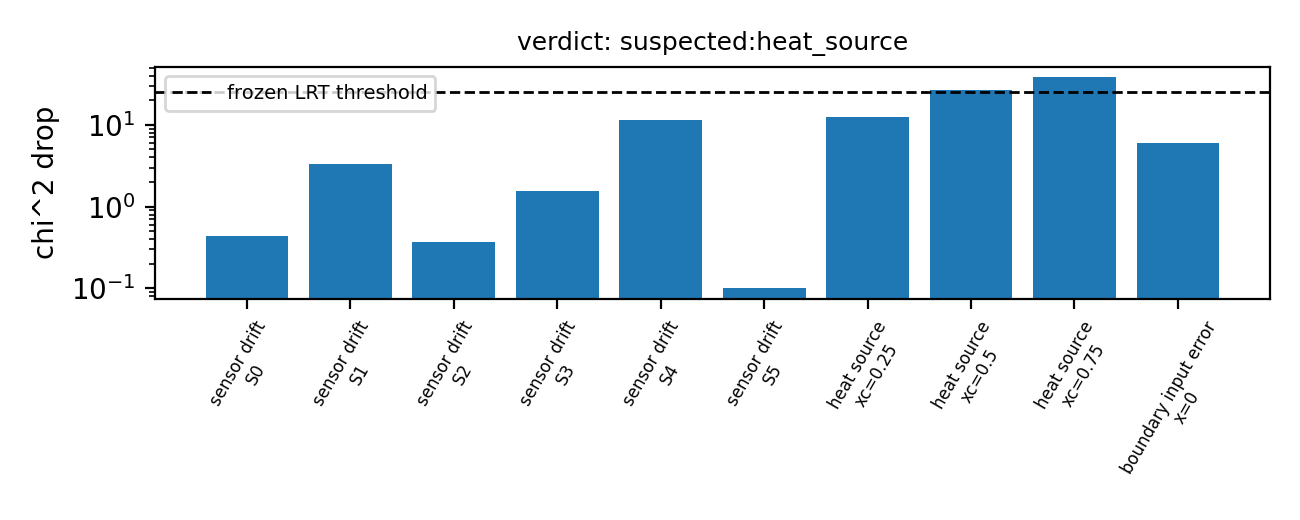
\includegraphics[width=0.48\linewidth]{diagnosis}\hfill
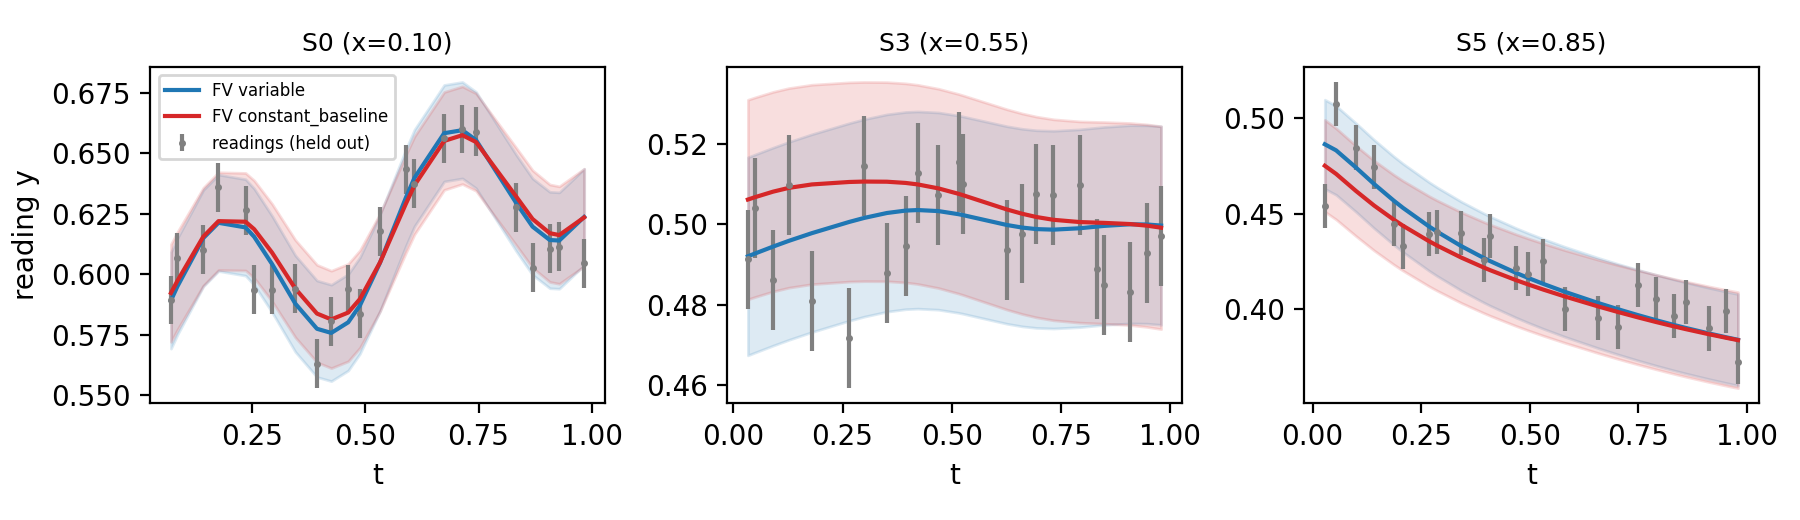
\includegraphics[width=0.50\linewidth]{val_predictions}
\caption{(a) Sealed blind test: $\Delta\chi^2$ per hypothesis vs frozen threshold. (b) Held-out E4\syn:
readings vs FV variable (blue) and constant (red) predictions with 95\% reading intervals.}\label{fig:s4}
\end{figure}

\textbf{Recovery and visibility.} Checkpoints carry a fingerprint (config + data hash); writes are
atomic. A run killed mid-training and resumed reproduces the uninterrupted parameters exactly
(max difference \RestartDiff); a checkpoint from another config is refused; a truncated newest file is
skipped; an injected non-finite loss is logged, rolled back and the lr halved (\RestartAll). Every
result JSON logs data sha256, config + hash, seed, git commit/dirty flag, hardware, threads, versions,
wall time.

\textbf{One misleading result, investigated.} In the first public evaluation a PINN seed passed the
recheck with $h{=}\VOneSeedTwoH$ (true \TrueH): $\chi^2_\nu{=}\VOneSeedTwoChi$ against a limit of
\VOneSeedTwoLim. Investigation: an absolute $\chi^2_\nu$ test has little power because a wrong $h$ moves
$\chi^2_\nu$ by $\sim$0.1. Fix: test the PINN parameters against the FV optimum on the same data
(LRT, $\chi^2_k$); it rejects this case by a wide margin and is pinned by a regression test.
Testing also found four input bugs (IDs restarting per experiment were all dropped as conflicts; a
NaN input passed silently; unknown flags were trusted; per-experiment query IDs were rejected), all fixed.

\textbf{Compute.} Laptop i7-1165G7 (4 cores), 16\,GB, no GPU, 4 torch threads. FV fit \FvFitSec\,s;
PINN \PinnTrainSec\,s/seed + \PinnAdaptSec\,s physics-only adaptation; full public evaluation \EvalWall\,min;
CPU smoke run of every stage \SmokeMin\,min (\SmokeOk; budget 10\,min).

\section{Claims, limitations, time}
\textbf{Supported\syn:} FV recovery with calibrated intervals under the stated noise model; $h$ is the
weakly identified parameter and a Robin-end sensor improves its precision; guards detect
dependent noise, wrong diffusivity form, PINN parameter inconsistency and three fault types above
measured sizes. \textbf{Not supported / unresolved:} anything on real data; faults below the
detection limits bias $\beta$ silently; Laplace intervals are local; the PINN's $h$; design accuracy
gain (only precision shown); coverage from 20 datasets. \textbf{Distinctions kept:} training fit
(Table~\ref{tab:main} row 5) vs held-out prediction (rows 6--7) vs parameter recovery (synthetic only)
vs physical consistency (energy balance, PINN--FV agreement).
\textbf{Time spent:} build and experiments $\approx$5\,h (24 Oct 21:50 -- 25 Oct 02:30 IST, AI-assisted);
review and walkthrough preparation on 25 Oct (author).

\newpage
\section*{Appendix --- AI assistance and verification (1 page)}
\textbf{How AI was used.} Claude (Anthropic) was used as a pair-programmer throughout, as the brief
permits: drafting code, running experiments, and drafting this report. I directed the plan,
decisions and trade-offs; the AI proposed and implemented them; decisions such as dropping PINN tuning,
adding guards and tightening thresholds were discussed and approved explicitly.

\textbf{How the output was verified --- by evidence, not trust.}
\begin{itemize}
\item \emph{Independent references:} the solver is checked against a manufactured solution (hand-derived
source), a closed-form steady state, discrete energy conservation and the maximum principle; the PINN
operator is checked against the same hand-derived source.
\item \emph{Known truth:} recovery, coverage, ablation, design and diagnosis studies use synthetic data with
truth stored separately and read only for scoring; a monkeypatched file guard proves fit/predict never
open it; corrupting validation labels leaves training estimates bit-identical.
\item \emph{Pre-registration:} methods and diagnosis rules were committed before the final evaluation and
the sealed blind test; the git history shows the order. Rule changes (one-sided autocorrelation test,
Bonferroni threshold) are declared with the evidence that motivated them.
\item \emph{Adversarial testing:} 56 automated tests (black-box: metamorphic shift/scale invariance,
renamed IDs/layouts, row order, edge-of-box truths, malformed inputs, CLI; white-box: autograd operator,
Jacobian, decision branches, interval algebra). They found four real bugs and one wrong test premise.
\item \emph{AI errors caught:} an ad-hoc threshold, a guard with too little power, a premature claim that a
status rule was protective (it let a 9$\times$ error through), a mis-stated clock time. Each was challenged,
re-measured and corrected; the over-engineering review removed dead code and test hooks from production paths.
\item \emph{No hand-typed numbers:} every number in this report is generated from result files by
\texttt{report/make\_numbers.py}.
\end{itemize}
\end{document}
